
\usetikzlibrary{shapes.geometric, positioning, arrows.meta, matrix}

\begin{figure}[H]
\centering
\large $G = (\{0, 1, 2, 3\}, \{(0, 1), (0, 2), (2, 1), (3, 2)\})$
\vspace{6mm}

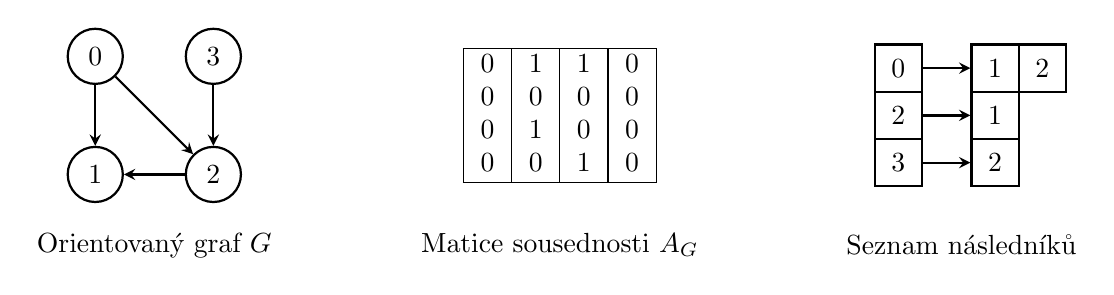
\begin{tikzpicture}[
  vnode/.style={circle, draw, minimum size=7mm, inner sep=0pt},
  boxnode/.style={rectangle, draw, minimum size=6mm, inner sep=0pt, anchor=center},
  thick,
  >=stealth
]
  % (a) Orientovaný graf G
  \begin{scope}[shift={(0,0)}]
    \node[vnode] (0) at (0, 1.5) {0};
    \node[vnode] (3) at (1.5, 1.5) {3};
    \node[vnode] (1) at (0, 0) {1};
    \node[vnode] (2) at (1.5, 0) {2};

    \draw[->] (0) -- (1);
    \draw[->] (0) -- (2);
    \draw[->] (3) -- (2);
    \draw[->] (2) -- (1);

    \node at (0.75, -0.9) {Orientovaný graf $G$};
  \end{scope}

  % (b) Matice sousednosti A_G
  \begin{scope}[shift={(5.0,0)}]
    \node (m) at (0.9,0.75) {
      \begin{tabular}{|c|c|c|c|}\hline
      0 & 1 & 1 & 0 \\
      0 & 0 & 0 & 0 \\
      0 & 1 & 0 & 0 \\
      0 & 0 & 1 & 0 \\\hline
      \end{tabular}
    };

    % Popisky řádků a sloupců (removed due to matrix replacement)

    \node at (0.9, -0.9) {Matice sousednosti $A_G$};
  \end{scope}

  % (c) Seznam následníků
  \begin{scope}[shift={(10.2,0)}]
    % Levý sloupec vrcholů (0, 2, 3)
    \node[boxnode] (h0) at (0, 1.35) {0};
    \node[boxnode, below=-\pgflinewidth of h0] (h2) {2};
    \node[boxnode, below=-\pgflinewidth of h2] (h3) {3};

    % Řádek 0:
    \node[boxnode, right=6mm of h0] (l01) {1};
    \node[boxnode, right=-\pgflinewidth of l01] (l02) {2};
    \draw[->] (h0) -- (l01);

    % Řádek 2:
    \node[boxnode, right=6mm of h2] (l21) {1};
    \draw[->] (h2) -- (l21);

    % Řádek 3:
    \node[boxnode, right=6mm of h3] (l32) {2};
    \draw[->] (h3) -- (l32);

    \node at (0.8, -0.9) {Seznam následníků};
  \end{scope}

\end{tikzpicture}
\caption{Orientovaný graf $G$ a jeho reprezentace maticí sousednosti a seznamem následníků.}
\label{fig:orientovany-graf-reprezentace}
\end{figure}
